\documentclass[12pt, twoside]{article}
%\documentclass[12pt, twoside]{article}
\usepackage[letterpaper, margin=1in, headsep=0.2in]{geometry}
\setlength{\headheight}{0.6in}
%\usepackage[english]{babel}
\usepackage[utf8]{inputenc}
\usepackage{microtype}
\usepackage{amsmath}
\usepackage{amssymb}
%\usepackage{amsfonts}
\usepackage[nomessages]{fp} %\FPeval{\var-name}{2*sin(pi/6)}
\usepackage{siunitx} %units in math. eg 20\milli\meter
\usepackage{yhmath} % for arcs, overparenth command
\usepackage{tikz} %graphics
\usetikzlibrary{quotes, angles, arrows, arrows.meta}
\usepackage{pgfplots}
\usepgfplotslibrary{fillbetween}
\pgfplotsset{compat=1.16}
\usepackage{graphicx} %consider setting \graphicspath{{images/}}
\usepackage{parskip} %no paragraph indent
\usepackage{enumitem}
\usepackage{multicol}
\usepackage{venndiagram}

\usepackage{fancyhdr}
\pagestyle{fancy}
\fancyhf{}
\renewcommand{\headrulewidth}{0pt} % disable the underline of the header
\raggedbottom
\hfuzz=2mm %suppresses overfull box warnings

\usepackage{hyperref}

\fancyhead[LO]{La Scuola d'Italia / Dr.\ Huson / IB Math 12 \\* 21 October 2026}
\fancyhead[RO]{\fbox{\begin{minipage}{6cm}\footnotesize Nickname:\\[0.5cm]\end{minipage}}}
\fancyfoot[C]{\thepage}

\begin{document}
\subsubsection*{2.3 Classwork: The Sine Rule and the Area of a Triangle}

\begin{center}
\fbox{\begin{minipage}{0.9\textwidth}
\centering
In triangle $ABC$, side $a$ is opposite angle $A$, side $b$ is opposite
angle $B$, and so on.
$$\frac{a}{\sin A} = \frac{b}{\sin B} = \frac{c}{\sin C}
\qquad\qquad
\text{Area} = \frac{1}{2}ab\sin C$$
\end{minipage}}
\end{center}

Give answers correct to three significant figures, unless they are exact.

\begin{enumerate}[itemsep=0.15cm]

%--- Problem 1: Sine rule for a side (AAS), area after third angle, sine rule for an acute angle (SSA), area SAS exact, angle from area [11 marks] ---
%--- Source: Original (freshly authored, AA SL 3.2); Haese AA SL Ch. 9 ---
\item[1.]
The diagrams are not to scale.

\begin{center}
\begin{tikzpicture}[scale=0.3]
  \coordinate (A) at (0,0);
  \coordinate (B) at (12.02,0);
  \coordinate (C) at (8.641,7.250);
  \draw[thick] (A) -- (B) -- (C) -- cycle;
  \draw pic["$40^\circ$", draw, angle radius=0.6cm, angle eccentricity=1.7] {angle = B--A--C};
  \draw pic["$65^\circ$", draw, angle radius=0.5cm, angle eccentricity=1.8] {angle = C--B--A};
  \node[below left] at (A) {$A$};
  \node[below right] at (B) {$B$};
  \node[above] at (C) {$C$};
  \node[above right] at (10.33,3.625) {$8$};
  \node[below] at (6,-1.6) {(a), (b)};
\end{tikzpicture}
\hfill
\begin{tikzpicture}[scale=0.3]
  \coordinate (P) at (0,0);
  \coordinate (Q) at (10,0);
  \coordinate (R) at (11.28,7.897);
  \draw[thick] (P) -- (Q) -- (R) -- cycle;
  \draw pic["$35^\circ$", draw, angle radius=0.7cm, angle eccentricity=1.6] {angle = Q--P--R};
  \node[below left] at (P) {$P$};
  \node[below right] at (Q) {$Q$};
  \node[above] at (R) {$R$};
  \node[below] at (5,0) {$10$};
  \node[right] at (10.64,3.95) {$8$};
  \node[below] at (5.6,-1.6) {(c)};
\end{tikzpicture}
\hfill
\begin{tikzpicture}[scale=0.3]
  \coordinate (K) at (0,0);
  \coordinate (L) at (9,0);
  \coordinate (M) at (5.196,3);
  \draw[thick] (K) -- (L) -- (M) -- cycle;
  \draw pic["$30^\circ$", draw, angle radius=0.8cm, angle eccentricity=1.55] {angle = L--K--M};
  \node[below] at (4.5,0) {$9$};
  \node[above left] at (2.598,1.5) {$6$};
  \node[below] at (4.5,-1.6) {(d)};
\end{tikzpicture}
\end{center}

\begin{enumerate}[itemsep=0.1cm]
  \item Find the length $AC$.
  \item Find the area of triangle $ABC$.
  \item In triangle $PQR$, angle $R$ is acute. Find the size of angle $R$.
  \item Find the exact area of the third triangle.
  \item A different triangle has two sides of length $5\,\text{cm}$ and
  $10\,\text{cm}$, and its area is $20\,\text{cm}^{2}$. The angle between
  these two sides is acute. Find the size of this angle.
\end{enumerate}

\begin{tikzpicture}
  \draw (-0.6,0) rectangle (14.6,7.4);
  \foreach \y in {1,2,...,7} \draw[dotted] (0,\y)--(14.1,\y);
\end{tikzpicture}

\newpage

%--- Problem 2: River width: third angle, sine rule for AT, right-angle trig for width, area of ABT; garden angle from area [9 marks] ---
%--- Source: Original (freshly authored, AA SL 3.2, 3.3); Haese AA SL Ch. 9 ---
\item[2.]
Points $A$ and $B$ are $200\,\text{m}$ apart on the straight bank of a
river. A tree $T$ stands on the opposite bank. Angle $TAB = 52^\circ$ and
angle $TBA = 71^\circ$. The two banks are parallel.

\begin{center}
\begin{tikzpicture}[scale=1.1]
  \coordinate (A) at (0,0);
  \coordinate (B) at (5,0);
  \coordinate (T) at (3.47,4.44);
  \coordinate (F) at (3.47,0);
  \draw[thick] (-1,0) -- (6.5,0);
  \draw[thick] (-1,4.44) -- (6.5,4.44);
  \draw (A) -- (T) -- (B);
  \draw[dotted, thick] (T) -- (F);
  \draw pic[draw, angle radius=0.2cm] {right angle = A--F--T};
  \draw pic["$52^\circ$", draw, angle radius=0.7cm, angle eccentricity=1.45] {angle = B--A--T};
  \draw pic["$71^\circ$", draw, angle radius=0.5cm, angle eccentricity=1.6] {angle = T--B--A};
  \node[below] at (A) {$A$};
  \node[below] at (B) {$B$};
  \node[above] at (T) {$T$};
  \node[below] at (2.5,0) {$200\,\text{m}$};
  \node[right] at (6.6,2.2) {river};
  \node[below right] at (6.6,-0.1) {\emph{not to scale}};
\end{tikzpicture}
\end{center}

\begin{enumerate}[itemsep=0.1cm]
  \item Write down the size of angle $ATB$.
  \item Find the distance $AT$.
  \item Find the width of the river.
  \item Find the area of triangle $ABT$.
\end{enumerate}

A triangular garden has two sides of length $8\,\text{m}$ and $10\,\text{m}$.
Its area is $30\,\text{m}^{2}$, and the angle between these two sides is
acute.

\begin{enumerate}[itemsep=0.1cm]
  \item[(e)] Find the size of the angle between the two sides.
\end{enumerate}

\begin{tikzpicture}
  \draw (-0.6,0) rectangle (14.6,8.4);
  \foreach \y in {1,2,...,8} \draw[dotted] (0,\y)--(14.1,\y);
\end{tikzpicture}

\end{enumerate}
\end{document}
